\documentclass{article}
\usepackage{tikz}
\usetikzlibrary{angles, quotes}
\usepackage{amssymb}
\usepackage{pgfplots}
\pgfplotsset{width=10cm,compat=1.9}
\usepgfplotslibrary{statistics}
\usepackage[left=2.54cm,right=2.54cm,top=2.54cm,bottom=2.54cm]{geometry}
\usepackage{tasks} %Paquete necesario para la producción de items horizontales para algunos ejercicios de tarea empleando el comando /begin{multicols}}{#}.../end{multicols} para ayudarnos a reducir las páginas
\usepackage{pdflscape} %comando que permite cambiar a orientación horizontal las hojas%
\usepackage{soul} %Paquete para permitir la compilación de acentos usando el comando {\hl{}}}\\
\sethlcolor{yellow(munsell)} %comando para definir el color para el subrayado usando el comando \hl
\usepackage[utf8]{inputenc}
\usepackage[spanish]{babel}
\usepackage{icomma}
\usepackage{ragged2e}
\usepackage{siunitx}
\usepackage{url}
\usepackage[colorlinks=true, urlcolor=blue,  linkcolor=black, citecolor=green]{hyperref}
\usepackage{pdfpages}
\usepackage{blindtext} %Paquete que genera texto ficticio (dummy text) con el comando: \blindtext
\usepackage{cancel} %in the preamble gives you four different modes of striking through: \cancel{text to cancel} draws a diagonal line (slash) through its argument, \bcancel{text to cancel} uses the negative slope (a backslash), \xcancel{text to cancel} draws an X (actually \cancel plus \bcancel), \cancelto{〈value〉}{〈expression〉} draws a diagonal arrow through the 〈expression〉pointing to the 〈value〉 (math-mode only)
\usepackage{csquotes}
\usepackage{afterpage}
\usepackage{parskip} 
\usepackage{float}
\usepackage{enumitem}
\usepackage{multicol}%Paquete que permite la creación aislada de columnas de texto. De esta forma se reduce la cantidad de páginas en nuestro documento
\usepackage{lipsum} %Paquete que genera texto de relleno al igual que \usepackage{blindtext}, se usa con el comando \lipsum[#-#] los #(hashtags) delimitan el número de páginas que deseamos ocupar del paquete lipsum para usarlos como relleno. 

% Definir el comando personalizado para la nota
\newcommand{\mynote}[1]{%
\begin{tikzpicture}[baseline=-0.75ex]
\node[draw, circle, fill=Apple Green!60, inner sep=2pt] (note) {\textbf{Nota:}};
\end{tikzpicture}%
\ \textit{#1}%
}

\newenvironment{Figura}
{\par\medskip\noindent\minipage{\linewidth}}
{\endminipage\par\medskip}
\usepackage{caption}
\usepackage[
backend=biber,
sorting=none,
url=true
]{biblatex} %bibliografía
\addbibresource{biblio.bib}
% Establecer el espacio entre las entradas de la bibliografía
\setlength{\bibitemsep}{1\baselineskip} % Puedes ajustar el valor según tus preferencias
\usepackage{amsmath,amsthm,amssymb,amsfonts}
\usepackage{pifont} %Permite la compilación del comando \xmark: es el símbolo de la tachita
\usepackage{mathtools} %permite la compilación de símbolos para matrices
\usepackage{empheq} %Paquete que se relaciona con \usepackage[most]{tcolorbox} para la creación de cuadros/cajas de colores para delimitar los resultados matemáticos o líneas de texto usando la línea de comando: \begin{empheq}[box={\mymath[colback=orange(webcolor)!70,drop lifted shadow]}]{equation*} \end{empheq}
\usepackage[most]{tcolorbox} %Paquete que se relaciona con \usepackage{empheq} para la creación de cuadros/cajas de colores para delimitar los resultados matemáticos o líneas de texto
\renewcommand{\qedsymbol}{$\blacksquare$}
\usetikzlibrary{positioning,decorations.pathreplacing} %Paquete que permite la compilación de llaves para cuadros sinópticos (brace diagram) 
\usepackage{schemata} %The schemata package is designed just for these brace diagrams
\usepackage{booktabs}

\newcommand\AB[2]{\schema{\schemabox{#1}}{\schemabox{#2}}} %comando o paquete necesario para crear cuadros sinópticos

\newtcbox{\mymath}[1][]{%
nobeforeafter, math upper, tcbox raise base,
enhanced, colframe=blue!30!black,
colback=blue!30, boxrule=1pt,
#1} %Comando importante para encasillar los resultados matemáticos en cajas de diferentes colores, se relaciona con los paquetes \usepackage{empheq} y \usepackage[most]{tcolorbox} 

\newenvironment{sysmatrix}[1]
{\left(\begin{array}{@{}#1@{}}}
{\end{array}\right)}
\newcommand{\ro}[1]{%
\xrightarrow{\mathmakebox[\rowidth]{#1}}%
}
\newlength{\rowidth}% row operation width
\AtBeginDocument{\setlength{\rowidth}{3em}}  %Comando importante para laproducción de lineas de operaciones entre matrices, método de Gauss o Gauss Jordan se relaciona con \newenvironment{sysmatrix}

%formato para cambiar el horario a español
\usepackage[spanish]{datetime2}
\DTMsetdatestyle{spanish}

\renewcommand{\today}{\DTMdisplaydate{\the\year}{\the\month}{\the\day }{-1}}
%%%%%%%%%%%%%%%%%%%%%%%%%%%%%%%%%%%%%%%%%

\usepackage{datetime}
\newcommand{\mycurrenttime}{\xxivtime}

%%%%%%%%%%%%%%%%%%%%%%%%%%%%%%%%%%%%%%%%%%%%%%%%%%%%%%%%%%%%%%%%%%%%%%%%%%%%%%%%%%%%%%%%%%%%%%%%%%%%%%%%%%%%%%%%%%%%%%%%%%%%%%%%%%%%%%%%%%%%%%%%%


%%%%%%%%%%%%%Caja de color para el título%%%%%%%%%%%%%%%%%%%%%%%%%%%%%%%%%%%%%%%%%%%%%%%%%%%%%%

\definecolor{myframecolor}{RGB}{1, 45, 75} % Prussian Blue
\definecolor{myboxcolor}{RGB}{0, 107, 92} % Apple Green

\newtcolorbox{mybox}{
enhanced,
colback=myboxcolor!7, % Color de fondo del cuadro
colframe=myframecolor, % Color del marco del cuadro
arc=0pt,
boxrule=1pt,
borderline west={2mm}{-10mm}{myframecolor}, % Borde en el lado izquierdo
sharp corners=southwest,
width=\linewidth,
before=\par\vspace{\bigskipamount}, % Espacio antes del cuadro
after=\par\vspace{\bigskipamount} % Espacio después del cuadro
}


\newcommand{\euler}{e} %Comando para producir letra e de euler
\newenvironment{remark}{\par\vfill\footnotesize % Vertical white space above the remark and smaller font size
\begin{list}{}{
	\leftmargin=80pt % Indentation on the left
	\rightmargin=60pt}\item\ignorespaces % Indentation on the right
\makebox[-2.5pt]{\begin{tikzpicture}[overlay]
		\node[draw=Horizon!60,line width=2.5pt,circle,fill=Horizon!25,font=\sffamily\bfseries,inner sep=4pt,outer sep=0pt] at (-19pt,5pt){\textcolor{Horizon}{Nota}};\end{tikzpicture}} % Blue Nota in a circle
\advance\baselineskip -1pt}{\end{list}\vskip5pt} % Tighter line spacing and white space after remark
\usepackage{graphicx}

\usepackage{titling}

\input{colores.tex}

%%Producir signos de cita textual``Asignatura''

\newcommand{\xmark}{\ding{55}} %%%comando que genera la tachita

\newenvironment{MyColorPar}[1]{%
\leavevmode\color{#1}\ignorespaces%
}{%
}%

%%%%%%%%%%%%%%%%%%% Título de la tarea, Nombre de alumno

\title{\textcolor{Apple Green}{\textbf{Tarea}} \textcolor{Sun}{\textbf{\#}}\textcolor{Cinnabar}{\textbf{1}} - \textbf{Termo}}
\author{\emph{Julio Alfredo Ballinas García} $\boldsymbol{\mid}$ 202107583}
\date{\today}

%%%%%%%%%%%%%%%%%%% Datos de la Materia

\usepackage{fancyhdr}
\fancypagestyle{plain}{%  the preset of fancyhdr 
\fancyhf{} % clear all header and footer fields
\fancyfoot[R]{
\includegraphics[width=2cm]{LogoFCFMBUAP (1).png}}
\fancyfoot[L]{{\bfseries{\thedate{}}} a las {\bfseries{\mycurrenttime{}}} horas{} (GMT-6, H. Puebla de Zaragoza, Pue)}
\fancyhead[L]{Mecánica Estadística (NRC: 22362)}
\fancyhead[R]{\theauthor}
}
\makeatletter
\def\@maketitle{%
\newpage
\null
\vskip 1em%
\begin{center}%
\let \footnote \thanks
{\LARGE \@title \par}%
\vskip 1em%
%{\large \@date}%
\end{center}%
\par
\vskip 1em}
\makeatother

\usepackage{lipsum}  
\usepackage{cmbright}


%%%%%%%%%%%%%%%%%%%%%%%%%%%%%%%%%%%%%%%%%%%%%%%%%%%%%%%%%%%%%%%%%%%%%%%%%%%%%%%%%%%%%%%%%%%%%%%%%%%%%%%%%%%%%%%%%%%%%%%%%%%%%%%%%%%%%%%%%%%%%%%%%%%%%%%%%%%%%%%%%%%%%%%%%%%%%%%%%%%%%%%%%%%%%%%%%%%%%%

% ========= Encabezado tipo artículo + Abstract box =========
% Metadatos simples (rellénalos en el cuerpo)
\newcommand{\PaperTitle}{}        % \PaperTitle{...}
\newcommand{\PaperAuthors}{}      % \PaperAuthors{Autor1$^{a}$, Autor2$^{b}$}
\newcommand{\PaperAffils}{}       % \PaperAffils{$^{a}$ Afiliación A\\ $^{b}$ Afiliación B}
\newcommand{\PaperDates}{}        % \PaperDates{Recibido..., Revisado..., Aceptado...}
\newcommand{\PaperJournal}{}      % \PaperJournal{Food Chemistry 108 (2008) 310–315}

% Caja de encabezado (título, autores, afiliaciones, fechas)
\newtcolorbox{articleheader}{
  enhanced, colback=white, colframe=black!60,
  boxrule=0.6pt, arc=0pt,
  left=6mm, right=6mm, top=4mm, bottom=4mm,
  borderline west={2mm}{0pt}{black!70},
  before skip=6pt, after skip=10pt
}

% Caja de Abstract (con título “Abstract” al estilo revista)
\newtcolorbox{abstractbox}[1][]{
  enhanced, colback=black!3, colframe=black!60,
  boxrule=0.6pt, arc=0pt,
  left=6mm, right=6mm, top=4mm, bottom=4mm,
  title=\textbf{Abstract}, fonttitle=\bfseries,
  attach boxed title to top left={xshift=6mm, yshift*=-2mm},
  boxed title style={colback=white, colframe=black!60, boxrule=0.6pt, arc=0pt},
  before skip=6pt, after skip=6pt,
  #1
}

% Comando para “Keywords”
\newcommand{\keywords}[1]{%
  \par\smallskip\noindent\textbf{Keywords:} \textit{#1}\par
}


%%%%%%%%%%%%%%%%%%%%%%%%%%%%%%%%%%%%%%%%%%%%%%%%%%%%%%%%%%%%%%%%%%%%%%%%%%%%%%%%%%%%%%%%%%%%%%%%%%%%%%%%%%%%%%%%%%%%%%%%%%%%%%%%%%%%%%%%%%%%%%%%%%%%%%%%%%%%%%%%%%%%%%%%%%%%%%%%%%%%%%%%%%%%%%%%%%%%%%%%%%

\begin{document}



\maketitle


%%%%%%%%%%%%%%%%%%% Datos del profesor, campus y aula

\begin{mybox}
\noindent\begin{tabular}{@{}ll}
	{\bfseries{Profesor}} & Dr. Jorge Velázquez Castro\\
	\textcolor{prussianblue}{\bfseries{Campus}} / \textcolor{trueblue}{\bfseries{Facultad}}  & \textcolor{prussianblue}{\bfseries{C.U. BUAP}} /  \textcolor{trueblue}{\bfseries{FCFM}} \\
	\textcolor{prussianblue}{\bfseries{Edificio}} /  \textcolor{trueblue}{\bfseries{Salón}}    & 	\textcolor{prussianblue}{\bfseries{EMA4}} /  \textcolor{trueblue}{\bfseries{407}}   
\end{tabular} 
\end{mybox} \vspace{1cm}

\section{Instrucciones de la tarea}
\addcontentsline{toc}{section}{Instrucciones de la tarea}


\setlength{\columnsep}{2cm}
\begin{multicols}{2}


% =====================
% Problema 1
% =====================
\begin{enumerate}[label={{\textcolor{trueblue}{\textbf{Ej}. \arabic*.0}}}, start=1]
\item \textbf{Problema 1: Tres cilindros con émbolos}
Tres cilindros están equipados con cuatro pistones, como se muestra en la figura. Las áreas de sección transversal de los cilindros están en la razón $A_1 : A_2 : A_3 = 1 : 2 : 3$. Los pares de pistones están acoplados de modo que sus desplazamientos son iguales. Las paredes de los cilindros son diatérmicas y están conectadas por una barra conductora de calor. El sistema completo está aislado. Encuentra las razones de presiones en los tres cilindros.


% Imagen del problema 1
\begin{center}
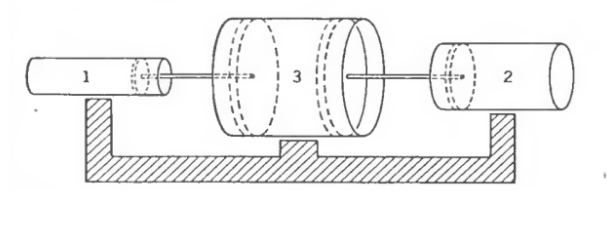
\includegraphics[width=1.3\linewidth]{tres_cilindros.png}
\end{center}
\end{enumerate}


% =====================
% Problema 2
% =====================
\begin{enumerate}[label={{\textcolor{trueblue}{\textbf{Ej}. \arabic*.0}}}, start=2]
\item \textbf{Problema 2: Ecuaciones de estado}


Encuentra las tres ecuaciones de estado de un sistema cuya ecuación fundamental es
\[
U = \left( \frac{v_0 \theta}{R^2} \right) \frac{S^3}{NV}
\]
Comprueba que las ecuaciones de estado son homogéneas de grado cero.
\end{enumerate}


% =====================
% Problema 3
% =====================
\begin{enumerate}[label={{\textcolor{trueblue}{\textbf{Ej}. \arabic*.0}}}, start=3]
\item \textbf{Problema 3: Ecuación fundamental}


Un sistema obedece las siguientes ecuaciones de estado:
\[
U = \tfrac{1}{2}PV, \qquad T^2 = \frac{AU^{3/2}}{VN^{1/2}}.
\]
Encuentra la ecuación fundamental.
\end{enumerate}


% =====================
% Problema 4
% =====================
\begin{enumerate}[label={{\textcolor{trueblue}{\textbf{Ej}. \arabic*.0}}}, start=4]
\item \textbf{Problema 4: Potencial químico}


Encuentra $\mu$ como función de $P$ y $T$ para el sistema con ecuación fundamental
\[
U = \left( \frac{v_0^2 \theta}{R^3} \right) \frac{S^4}{NV^2}.
\]

de donde $v_{0}$, $\theta$ y $R$ son constantes positivas. (\textbf{Nota}: Puede utilizar la ecuación de Gibbs-Duhem o  bien pasar a la representación conveniente)
\end{enumerate}


% =====================
% Problema 5
% =====================
\begin{enumerate}[label={{\textcolor{trueblue}{\textbf{Ej}. \arabic*.0}}}, start=5]
\item \textbf{Problema 5: Función de Massieu}


\textcolor{trueblue}{\textbf{Ej.}} \textcolor{trueblue}{5.1} Obtén la función de Massieu de variables naturales $(1/T,V,N)$ i.e. $S[1/T,V,N]$ de la ecuación fundamental del problema anterior.


\textcolor{trueblue}{\textbf{Ej.}} \textcolor{trueblue}{5.2} Obtén la función de Massieu de variables naturales $(1/T,V,\mu/T)$ i.e. $S[1/T,V,\mu/T]$ de la ecuación fundamental del problema 4. 
\end{enumerate}


% =====================
% Problema 6
% =====================
\begin{enumerate}[label={{\textcolor{trueblue}{\textbf{Ej}. \arabic*.0}}}, start=6]
\item \textbf{Problema 6: Calores específicos}


Encuentra el calor específico a presión constante y el calor específico a volumen constante del gas ideal monoatómico ($c=3/2$).
\end{enumerate}


% =====================
% Problema 7
% =====================
\begin{enumerate}[label={{\textcolor{trueblue}{\textbf{Ej}. \arabic*.0}}}, start=7]
\item \textbf{Problema 7: Expansión adiabática}


Un sistema tiene la ecuación fundamental
\[
u = A v^{-2} e^{s/R}.
\]
Inicialmente se encuentra a temperatura $T_0$ y presión $P_0$. Se expande con $S$ constante hasta que la presión es la mitad de la inicial. ¿Cuál es la temperatura final?
\end{enumerate}


% =====================
% Problema 8
% =====================
\begin{enumerate}[label={{\textcolor{trueblue}{\textbf{Ej}. \arabic*.0}}}, start=8]
\item \textbf{Problema 8: Equilibrio térmico}


Dos sistemas cumplen con las ecuaciones
\[
\frac{1}{T^{(1)}} = \tfrac{3}{2}R\frac{N^{(1)}}{U^{(1)}}, \qquad \frac{1}{T^{(2)}} = \tfrac{5}{2}R\frac{N^{(2)}}{U^{(2)}}.
\]
Están separados con una pared diatérmica. Los números molares son  $N^{(1)}=2$, $N^{(2)}=3$, las temperaturas iniciales $T^{(1)}=250K$, $T^{(2)}=350K$. ¿Cuál es el valor de $U^{(1)}$, $U^{(2)}$ cuando se alcanza el equilibrio? ¿Cuál es la temperatura de equilibrio?
\end{enumerate}


% =====================
% Problema 9
% =====================
\begin{enumerate}[label={{\textcolor{trueblue}{\textbf{Ej}. \arabic*.0}}}, start=9]
\item \textbf{Problema 9: Adsorción}


La energía libre de Helmholtz de cierto gas es
\[
-kT \ln \left[ \left( \tfrac{eV}{N_g} \right)^{N_g} (\lambda T)^{3N_g/2} \right].
\]
donde k,$\lambda$ son constantes y $e$ es el número $e$. Dicho gas ocupa un volumen $V$, está a temperatura $T$ y tiene $N_{g}$ partículas.  El gas se pone en contacto con una superficie donde se adsorben las moléculas. La energía libre de las moléculas adsorbidas en la superficie está dada por:

\[
-kTN_s \ln[L^2] - N_s \epsilon_0.
\]

donde $[L^{2}]$ es el área de la superficie (esta variable juega el papel de parámetro extensivo análogo al volumen). Encuentra el número de moléculas adsorbidas por unidad de área $(N_{s}/L^{2})$.
\textbf{Nota 1}: Se asume que inicialmente la superficie no tenía moléculas adsorbidas. \\

\underline{Recuerde}: En equilibrio el valor del potencial químico del gas y de las moléculas adsorbidas tiene el mismo valor.\\

 \textit{Nota cultural}: La \underline{adsorción} es un proceso por el cual átomos, iones, moléculas de gases, líquidos o sólidos disueltos son atrapados o retenidos en una superficie, en contraposición a la absorción, que es un fenómeno de volumen. 
\end{enumerate}


\end{multicols}


\tableofcontents \newpage

\section*{Problema 1}
\addcontentsline{toc}{section}{Problema 1}

\textcolor{Cinnabar}{\textbf{Solución}}:

El esquema mostrado corresponde a tres cilindros numerados $1$, $2$ y $3$, cada uno con un pistón móvil. Los cilindros están conectados a través de una base común y unidos mediante una barra conductora de calor, lo que significa que con el paso del tiempo los tres alcanzan el mismo estado térmico. Los pistones no son independientes: se encuentran acoplados en pares, de modo que al desplazarse uno de ellos, su compañero se desplaza en la misma magnitud. Esta condición de \textcolor{trueblue}{desplazamientos iguales} es fundamental, pues limita la forma en la que cambian los volúmenes y asegura que las fuerzas que actúan sobre la varilla común deben compensarse exactamente.


\begin{figure}[H]
  \centering
  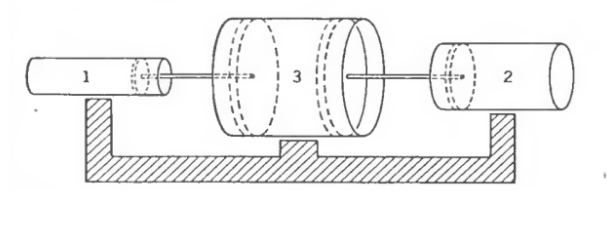
\includegraphics[width=0.85\linewidth]{tres_cilindros.png}
  \caption{Esquema del sistema: tres cilindros con áreas $A_1:A_2:A_3=1:2:3$ y dos pares de émbolos acoplados.}
  \label{fig:tres-cilindros}
\end{figure}

\medskip

Para empezar, conviene resaltar la información principal: las áreas de sección transversal de los cilindros se encuentran en la razón
\[
A_1 : A_2 : A_3 = 1 : 2 : 3.
\]
Esto significa que si el área del cilindro $1$ se toma como unidad, el área del cilindro $2$ es el doble y la del cilindro $3$ es el triple. Esta diferencia de tamaños se traduce directamente en diferencias de fuerzas, ya que la fuerza sobre un pistón es el producto de la presión interna por el área del émbolo:
\[
F_i = P_i A_i.
\]

\medskip

Al ser las paredes diatérmicas y existir la barra conductora, no hay forma de que un cilindro conserve una temperatura distinta a los otros. Después de un intercambio inicial de energía, los tres gases alcanzan el mismo valor:
\[
T_1 = T_2 = T_3.
\]
De esta manera, las comparaciones de presión que se van a establecer dependen únicamente de la condición de equilibrio mecánico en los acoplamientos.

\medskip

En el acoplamiento que une a los cilindros $1$ y $2$, la varilla transmite las fuerzas ejercidas por los gases sobre cada pistón.
De un lado actúa la presión interna del cilindro $1$, multiplicada por su área $A_1$; del otro, la presión del cilindro $2$ sobre el área $A_2$.
Dado que la varilla es perfectamente rígida y no tiene masa, no puede sostener una diferencia neta de fuerzas, de manera que el equilibrio obliga a que ambas contribuciones sean iguales:
\[
P_1 A_1 = P_2 A_2.
\]
Sustituyendo las razones de área se encuentra
\[
\frac{P_1}{P_2} = \frac{A_2}{A_1} = \frac{2}{1} = 2,
\]
lo cual indica que el gas del cilindro $1$ debe ejercer el doble de presión que el gas del cilindro $2$ para mantener a la varilla en equilibrio.

\medskip

El mismo razonamiento se aplica al segundo par de pistones, que conecta a los cilindros $2$ y $3$. Allí la condición de equilibrio sobre la varilla exige
\[
P_2 A_2 = P_3 A_3,
\]
y al sustituir las áreas
\[
\frac{P_2}{P_3} = \frac{A_3}{A_2} = \frac{3}{2}.
\]
De aquí se obtiene que la presión en el cilindro $2$ es una vez y media la presión en el cilindro $3$.

\medskip

Al combinar ambas relaciones, es posible obtener un cociente directo entre las presiones extremas de los cilindros $1$ y $3$:
\[
\frac{P_1}{P_3} = \frac{P_1}{P_2} \cdot \frac{P_2}{P_3} = 2 \cdot \frac{3}{2} = 3.
\]
La forma más sencilla de expresar todas las proporciones a la vez es escribirlas en números enteros:
\[
P_1 : P_2 : P_3 = 6 : 3 : 2.
\]

\medskip

Si en lugar del montaje recto los pistones estuvieran colocados con cierta inclinación respecto al eje de la varilla, 
la fuerza ejercida por cada gas no se transmitiría completamente en la dirección del acoplamiento, 
sino sólo su componente paralela. En ese caso, la condición de equilibrio adoptaría la forma  
\[
P_i A_i \cos\theta_i = P_j A_j \cos\theta_j,
\]  
donde $\theta$ es el ángulo de inclinación de cada pistón respecto al eje de transmisión. 
En el esquema actual los pistones trabajan alineados con la varilla, lo que equivale a $\theta = 0$ 
y por tanto $\cos\theta = 1$. De este modo, el término angular desaparece y las relaciones se reducen 
a las igualdades más simples entre $P_i A_i$ y $P_j A_j$. \vspace{0.5cm}

\section*{Problema 2}
\addcontentsline{toc}{section}{Problema 2}

\textcolor{Cinnabar}{\textbf{Solución}}:

En la \textbf{representación energética}, la \textcolor{orange(colorwheel)}{\textbf{energía interna}} se escribe como función de las variables extensivas:
\begin{equation}
U = U(S,V,N).
\label{eq:generalU}
\end{equation}

Al derivar de manera total:
\begin{equation}
\begin{split}
dU
&= \left( \frac{\partial U}{\partial S} \right)_{V,N} dS
 + \left( \frac{\partial U}{\partial V} \right)_{S,N} dV
 + \left( \frac{\partial U}{\partial N} \right)_{S,V} dN.
\end{split}
\label{eq:dU}
\end{equation}

De \eqref{eq:dU} se identifican directamente las variables intensivas:
\begin{equation}
\begin{split}
T &\equiv \left( \frac{\partial U}{\partial S} \right)_{V,N}
\quad\;\;\;\;\; \textcolor{Cerulean}{\text{(temperatura)}}, \\[6pt]
-P &\equiv \left( \frac{\partial U}{\partial V} \right)_{S,N}
\quad \textcolor{Cerulean}{\text{(presión)}}, \\[6pt]
\mu &\equiv \left( \frac{\partial U}{\partial N} \right)_{S,V}
\quad \textcolor{Cerulean}{\text{(potencial químico)}}.
\end{split}
\label{eq:defs}
\end{equation}

\subsection*{Planteamiento del problema}
\addcontentsline{toc}{subsection}{Planteamiento del problema}

La ecuación fundamental es:
\begin{equation}
U(S,V,N)=\left(\frac{v_0\,\theta}{R^2}\right)\frac{S^3}{N V}.
\label{eq:fundamental2}
\end{equation}

Definimos la constante:
\begin{equation}
K \;\equiv\; \frac{v_0 \theta}{R^2},
\qquad\Rightarrow\qquad
U=K\frac{S^3}{N V}.
\label{eq:Kdef}
\end{equation}

\subsection*{1) Ecuaciones de estado}
\addcontentsline{toc}{subsection}{1) Ecuaciones de estado}

\textbf{Temperatura:}  
De \eqref{eq:Kdef}:
\begin{equation}
\begin{split}
T &= \left(\frac{\partial U}{\partial S}\right)_{V,N}
=K\frac{1}{N V}\frac{\partial}{\partial S}(S^3) \\[6pt]
&= K\frac{3 S^2}{N V}
= \frac{3}{S}\underbrace{\left(K\frac{S^3}{N V}\right)}_{U} \\[6pt]
&= \textcolor{Cerulean}{\frac{3U}{S}}.
\end{split}
\label{eq:T2}
\end{equation}

\textbf{Presión:}  
\begin{equation}
\begin{split}
\left(\frac{\partial U}{\partial V}\right)_{S,N}
&= K\frac{S^3}{N}\frac{\partial}{\partial V}\!\left(\frac{1}{V}\right) \\[6pt]
&= -K\frac{S^3}{N V^2}.
\end{split}
\end{equation}
Por \eqref{eq:defs}:
\begin{equation}
\begin{split}
P &= -\left(\frac{\partial U}{\partial V}\right)_{S,N}
=K\frac{S^3}{N V^2} \\[6pt]
&= \frac{1}{V}\underbrace{\left(K\frac{S^3}{N V}\right)}_{U}
= \textcolor{Cerulean}{\frac{U}{V}}.
\end{split}
\label{eq:P2}
\end{equation}

\textbf{Potencial químico:}  
\begin{equation}
\begin{split}
\left(\frac{\partial U}{\partial N}\right)_{S,V}
&= K\frac{S^3}{V}\frac{\partial}{\partial N}\!\left(\frac{1}{N}\right) \\[6pt]
&= -K\frac{S^3}{N^2 V}.
\end{split}
\end{equation}
Por \eqref{eq:defs}:
\begin{equation}
\begin{split}
\mu &= \left(\frac{\partial U}{\partial N}\right)_{S,V}
=-K\frac{S^3}{N^2 V} \\[6pt]
&= -\frac{1}{N}\underbrace{\left(K\frac{S^3}{N V}\right)}_{U} \\[6pt]
&= \textcolor{Cerulean}{-\frac{U}{N}}.
\end{split}
\label{eq:mu2}
\end{equation}

\textcolor{Tarawera}{\textbf{Resumen}}:
\begin{equation}
\boxed{T=\tfrac{3U}{S}, \quad P=\tfrac{U}{V}, \quad \mu=-\tfrac{U}{N}}
\label{eq:resumen}
\end{equation}

\subsection*{2) Homogeneidad}
\addcontentsline{toc}{subsection}{2) Homogeneidad}

De \eqref{eq:fundamental2}:
\begin{equation}
\begin{split}
U(\lambda S,\lambda V,\lambda N)
&= K\frac{(\lambda S)^3}{(\lambda N)(\lambda V)} \\[6pt]
&= \lambda\,K\frac{S^3}{N V}
=\lambda U(S,V,N).
\end{split}
\label{eq:homogeneidad}
\end{equation}

Por lo tanto, \(U\) es homogénea de grado uno, y de \eqref{eq:T2}, \eqref{eq:P2} y \eqref{eq:mu2} se confirma que \(T,P,\mu\) son homogéneas de grado cero.

\subsection*{3) Relación de Euler}
\addcontentsline{toc}{subsection}{3) Relación de Euler}

Comprobemos que se cumple
\begin{equation}
U = T S - P V + \mu N.
\label{eq:Euler}
\end{equation}

De \eqref{eq:T2}, \eqref{eq:P2}, \eqref{eq:mu2}:
\begin{equation}
\begin{split}
TS &= \tfrac{3U}{S}\,S = 3U, \\[6pt]
PV &= \tfrac{U}{V}\,V = U, \\[6pt]
\mu N &= -\tfrac{U}{N}\,N = -U.
\end{split}
\end{equation}

Entonces:
\begin{equation}
TS - PV + \mu N = 3U - U - U = U,
\end{equation}
con lo que se verifica \eqref{eq:Euler}.


\section*{Problema 3}
\addcontentsline{toc}{section}{Problema 3}

\textcolor{Cinnabar}{\textbf{Solución}}:

En la \textbf{representación energética}, la 
\textcolor{orange(colorwheel)}{\textbf{energía interna}} es función de variables extensivas:
\begin{equation}
U = U(S,V,N).
\label{eq:p3-U-general}
\end{equation}

La diferencial total es
\begin{equation}
\begin{split}
dU
&= \left( \frac{\partial U}{\partial S} \right)_{V,N} dS
 + \left( \frac{\partial U}{\partial V} \right)_{S,N} dV
 + \left( \frac{\partial U}{\partial N} \right)_{S,V} dN,
\end{split}
\label{eq:p3-dU}
\end{equation}
de donde identificamos
\begin{equation}
\begin{split}
T &\equiv \left( \frac{\partial U}{\partial S} \right)_{V,N},
\qquad
-P \equiv \left( \frac{\partial U}{\partial V} \right)_{S,N},
\qquad
\mu \equiv \left( \frac{\partial U}{\partial N} \right)_{S,V}.
\end{split}
\label{eq:p3-intensivas}
\end{equation}

\subsection*{Planteamiento}
\addcontentsline{toc}{subsection}{Planteamiento}

Se dan las ecuaciones de estado
\begin{equation}
U = \tfrac{1}{2}\,P V,
\qquad
T^{2} = \frac{A\,U^{3/2}}{V\,N^{1/2}},
\label{eq:p3-datos}
\end{equation}
con \(A>0\) constante. Buscamos \(U(S,V,N)\).

\subsection*{1) Relación entre \(U\) y \(V\)}
\addcontentsline{toc}{subsection}{1) Relación entre U y V}

De la primera de \eqref{eq:p3-datos}:
\begin{equation}
\begin{split}
U &= \tfrac{1}{2}PV 
\quad\Longrightarrow\quad
P = \frac{2U}{V}.
\end{split}
\label{eq:p3-P-en-UyV}
\end{equation}

Usando la definición de presión en \eqref{eq:p3-intensivas}:
\begin{equation}
\begin{split}
P &= -\left(\frac{\partial U}{\partial V}\right)_{S,N}
\quad\stackrel{\eqref{eq:p3-P-en-UyV}}{\Longrightarrow}\quad
\left(\frac{\partial U}{\partial V}\right)_{S,N} = -\frac{2U}{V}.
\end{split}
\label{eq:p3-edo-V}
\end{equation}

Separación de variables (a \(S,N\) fijos) e integración:
\begin{equation}
\begin{split}
\frac{1}{U}\left(\frac{\partial U}{\partial V}\right)_{S,N} &= -\frac{2}{V}
\quad\Longrightarrow\quad
\frac{\partial}{\partial V}\big(\ln U\big) = -\frac{2}{V} \\[4pt]
\Longrightarrow\quad
\ln U &= -2\ln V + f(S,N).
\end{split}
\label{eq:p3-int-V}
\end{equation}

Elevando y definiendo \(F(S,N)\equiv e^{f(S,N)}\!>\!0\):
\begin{equation}
U(S,V,N) = \frac{F(S,N)}{V^{2}}.
\label{eq:p3-U-factorizada}
\end{equation}

\subsection*{2) Relación entre \(U\) y \(S\)}
\addcontentsline{toc}{subsection}{2) Relación entre U y S}

De la segunda de \eqref{eq:p3-datos}:
\begin{equation}
T=\frac{\sqrt{A}\;U^{3/4}}{V^{1/2}N^{1/4}}.
\label{eq:p3-T-en-U}
\end{equation}
Pero por \eqref{eq:p3-intensivas}, \(T=\big(\partial U/\partial S\big)_{V,N}\).  
Sustituyendo \eqref{eq:p3-U-factorizada} en \eqref{eq:p3-T-en-U}:
\begin{equation}
\begin{split}
\left(\frac{\partial U}{\partial S}\right)_{V,N}
&= \frac{1}{V^{2}}\frac{\partial F}{\partial S}
= \frac{\sqrt{A}}{V^{1/2}N^{1/4}}\left(\frac{F}{V^{2}}\right)^{3/4} \\[4pt]
&= \frac{\sqrt{A}}{V^{1/2}N^{1/4}}\;\frac{F^{3/4}}{V^{3/2}}
= \frac{\sqrt{A}}{N^{1/4}}\;\frac{F^{3/4}}{V^{2}}.
\end{split}
\label{eq:p3-edo-S-previa}
\end{equation}
Multiplicando por \(V^{2}\):
\begin{equation}
F_{S}(S,N)=\frac{\sqrt{A}}{N^{1/4}}\,F(S,N)^{3/4}.
\label{eq:p3-edo-S}
\end{equation}

Separación e integración:
\begin{equation}
\begin{split}
\int F^{-3/4}\,dF
&= \int \frac{\sqrt{A}}{N^{1/4}}\,dS
\quad\Longrightarrow\quad
4\,F^{1/4}
= \frac{\sqrt{A}}{N^{1/4}}\,S + g(N).
\end{split}
\label{eq:p3-int-S}
\end{equation}
Escribimos
\begin{equation}
F^{1/4}(S,N) = \frac{\sqrt{A}}{4}\,\frac{S}{N^{1/4}} + h(N),
\label{eq:p3-F14}
\end{equation}
con \(h(N)=g(N)/4\).

\subsection*{3) Condición de extensividad}
\addcontentsline{toc}{subsection}{3) Condición de extensividad}

La energía interna es homogénea de grado uno:
\begin{equation}
U(\lambda S,\lambda V,\lambda N)=\lambda\,U(S,V,N).
\label{eq:p3-extensiva}
\end{equation}
A partir de \eqref{eq:p3-U-factorizada}–\eqref{eq:p3-F14} se requiere
\begin{equation}
h(N)\propto N^{3/4}.
\label{eq:p3-h-escala}
\end{equation}
Si además imponemos la condición física \(U\to 0\) cuando \(S\to 0\), tomamos \(h(N)=0\).  
Entonces, de \eqref{eq:p3-F14}:
\begin{equation}
F(S,N)=\left(\frac{\sqrt{A}}{4}\,\frac{S}{N^{1/4}}\right)^{4}
=\frac{A^{2}}{256}\,\frac{S^{4}}{N}.
\label{eq:p3-F-final}
\end{equation}
Sustituyendo en \eqref{eq:p3-U-factorizada}:
\begin{equation}
U(S,V,N)=\frac{A^{2}}{256}\;\frac{S^{4}}{N\,V^{2}}.
\label{eq:p3-U-final}
\end{equation}

\subsection*{4) Forma entropía}
\addcontentsline{toc}{subsection}{4) Forma entropía}

De \eqref{eq:p3-U-final} despejamos \(S\):
\begin{equation}
\begin{split}
U\,N\,V^{2}
&= \frac{A^{2}}{256}\,S^{4}
\quad\Longrightarrow\quad
S^{4}=\frac{256}{A^{2}}\,U\,N\,V^{2}.
\end{split}
\label{eq:p3-S4}
\end{equation}
Aplicando raíz cuarta:
\begin{equation}
S(U,V,N)=\left(\frac{256}{A^{2}}\,U\,N\,V^{2}\right)^{\!1/4}
=\frac{4}{\sqrt{A}}\;\big(U N V^{2}\big)^{1/4}.
\label{eq:p3-S-forma}
\end{equation}

\subsection*{5) Verificación}
\addcontentsline{toc}{subsection}{5) Verificación}

\textbf{Presión:}
\begin{equation}
\begin{split}
P
&= -\left(\frac{\partial U}{\partial V}\right)_{S,N}
= -\frac{\partial}{\partial V}\!\left(\frac{A^{2}}{256}\,\frac{S^{4}}{N\,V^{2}}\right)_{S,N} \\[4pt]
&= \frac{A^{2}}{256}\,\frac{2S^{4}}{N\,V^{3}}
= \frac{2}{V}\,
\underbrace{\left(\frac{A^{2}}{256}\,\frac{S^{4}}{N\,V^{2}}\right)}_{U}
= \frac{2U}{V},
\end{split}
\label{eq:p3-P-check}
\end{equation}
coincidiendo con \eqref{eq:p3-P-en-UyV}.

\textbf{Temperatura:}
\begin{equation}
\begin{split}
T
&= \left(\frac{\partial U}{\partial S}\right)_{V,N}
= \frac{A^{2}}{256}\,\frac{1}{N\,V^{2}}\;\frac{d}{dS}(S^{4}) \\[4pt]
&= \frac{A^{2}}{256}\,\frac{1}{N\,V^{2}}\,(4S^{3})
= \frac{A^{2}}{64}\,\frac{S^{3}}{N\,V^{2}}.
\end{split}
\label{eq:p3-T-check}
\end{equation}
Elevando al cuadrado y usando \eqref{eq:p3-S4}:
\begin{equation}
\begin{split}
T^{2}
&= \left(\frac{A^{2}}{64}\right)^{2}\frac{S^{6}}{N^{2}V^{4}}
= \frac{A^{4}}{4096}\,\frac{S^{2}}{N^{2}V^{4}}\,
\underbrace{S^{4}}_{\left(\frac{256}{A^{2}}U N V^{2}\right)} \\[4pt]
&= \frac{A^{2}}{16}\,\frac{S^{2}}{N\,V^{2}}\;\frac{U}{V^{2}}
= \frac{A^{2}}{16}\,\frac{1}{N\,V^{2}}
\left(\frac{256}{A^{2}}U N V^{2}\right)^{\!1/2}\frac{U}{V^{2}} \\[4pt]
&= \frac{A\,U^{3/2}}{V\,N^{1/2}},
\end{split}
\label{eq:p3-T2-check}
\end{equation}
que reproduce exactamente la segunda de \eqref{eq:p3-datos}.

\subsection*{Resultado}
\addcontentsline{toc}{subsection}{Resultado final}

\begin{empheq}[box={\mymath[colback=Apple Green!20,drop lifted shadow]}]{equation}
	\label{eq:phiP}
	\begin{split}
		\varphi(r) &=
		\frac{1}{4\pi\epsilon_{0}}
		\frac{ \mathbf{P} \cdot \bigl( \mathbf{r} - \mathbf{r}^{\prime} \bigr) }
		{ \left| \mathbf{r} - \mathbf{r}^{\prime} \right|^{3} }
	\end{split}
	\tag{2-39}
\end{empheq}




\section*{Problema 4}
\addcontentsline{toc}{section}{Problema 4}

\textcolor{Cinnabar}{\textbf{Solución}}:

El sistema tiene como ecuación fundamental:
\begin{equation}
U(S,V,N)=\left(\frac{v_{0}^{2}\theta}{R^{3}}\right)\frac{S^{4}}{N V^{2}}.
\label{eq:fundamental}
\end{equation}

Definamos la constante:
\begin{equation}
\textcolor{trueblue}{K \;\equiv\; \frac{v_{0}^{2}\theta}{R^{3}}}
\qquad\Rightarrow\qquad
U \;=\; K\,\frac{S^{4}}{N V^{2}}.
\label{eq:constanteK}
\end{equation}

Nuestro objetivo es expresar el \textcolor{Cerulean}{potencial químico $\mu$} como función de \(P\) y \(T\).

\subsection*{1) Variables intensivas por diferenciación}
\addcontentsline{toc}{subsection}{1) Variables intensivas por diferenciación}

De la ecuación \eqref{eq:constanteK} se obtienen las variables intensivas:

\textbf{Temperatura}:
\begin{equation}
T=\left(\frac{\partial U}{\partial S}\right)_{V,N}
=K\,\frac{1}{N V^{2}}\frac{\partial}{\partial S}(S^{4})
=\frac{4K}{N V^{2}}\,S^{3}.
\label{eq:T}
\end{equation}

\textbf{Presión}:
\begin{equation}
P=-\left(\frac{\partial U}{\partial V}\right)_{S,N}
=-K\,\frac{S^{4}}{N}\frac{\partial}{\partial V}\!\left(\frac{1}{V^{2}}\right)
=\frac{2K}{N}\,\frac{S^{4}}{V^{3}}.
\label{eq:P}
\end{equation}

\textbf{Potencial químico}:
\begin{equation}
\mu=\left(\frac{\partial U}{\partial N}\right)_{S,V}
=-\,K\,\frac{S^{4}}{N^{2}V^{2}}.
\label{eq:mu}
\end{equation}

\subsection*{2) Eliminación de $S$}
\addcontentsline{toc}{subsection}{2) Eliminación de $S$}

De la ecuación \eqref{eq:T}:
\begin{equation}
S^{3} = \frac{T\,N V^{2}}{4K}.
\label{eq:S3}
\end{equation}

De la ecuación \eqref{eq:P}:
\begin{equation}
S^{4} = \frac{P\,N V^{3}}{2K}.
\label{eq:S4}
\end{equation}

\subsection*{3) Expresión de $\mu(P,T)$}
\addcontentsline{toc}{subsection}{3) Expresión de $\mu(P,T)$}

Sustituyendo \eqref{eq:S4} en \eqref{eq:mu}:
\begin{equation}
\mu = -\,K\,\frac{1}{N^{2}V^{2}}
\left(\frac{P\,N V^{3}}{2K}\right)
= -\,\frac{P V}{2N}.
\label{eq:muPV}
\end{equation}

Para eliminar \(V/N\), combinamos \eqref{eq:S3} y \eqref{eq:S4}.  
Tomando la razón:
\begin{equation}
\frac{S^{4}}{S^{3}}=S
=\frac{\tfrac{P N V^{3}}{2K}}{\tfrac{T N V^{2}}{4K}}
=\frac{2 P V}{T}.
\label{eq:Sratio}
\end{equation}

De aquí se obtiene una relación entre \(S\), \(P\) y \(T\), que al sustituirse en \eqref{eq:muPV} permite expresar finalmente:
\begin{equation}
\mu(P,T) \;=\; -\,\frac{T}{4}\;\left(\frac{2T^{2}}{P}\right)^{1/3}.
\label{eq:muPT}
\end{equation}

\subsection*{Resultado final}
\addcontentsline{toc}{subsection}{Resultado final}

\begin{empheq}[box={\mymath[colback=Apple Green!20,drop lifted shadow]}]{equation}
\mu(P,T)
\;=\; -\,\frac{T}{4}\;\left(\frac{2T^{2}}{P}\right)^{1/3}.
\end{empheq}



\section*{Problema 5}
\addcontentsline{toc}{section}{Problema 5}

\textcolor{Cinnabar}{\textbf{Solución}}:

Este problema pide calcular la \textcolor{orange(colorwheel)}{\textbf{función de Massieu}}, que se obtiene como una 
\textbf{transformada de Legendre} de la entropía \(S\).  

\medskip

Si la entropía depende de variables extensivas \((U,V,N)\), entonces una 
transformada de Legendre respecto a la energía \(U\) da una nueva función con 
variables naturales \((1/T,V,N)\):
\begin{equation}
\Phi\!\left(\tfrac{1}{T},V,N\right)
= \max_{U}\,\Big(S(U,V,N)-\tfrac{1}{T}U\Big).
\label{eq:p5-Legendre}
\end{equation}

Análogamente, si se transforman \(U\) y \(N\), obtenemos variables naturales 
\((1/T,V,\mu/T)\):
\begin{equation}
\Psi\!\left(\tfrac{1}{T},V,\tfrac{\mu}{T}\right)
= \max_{U,N}\,\Big(S(U,V,N)-\tfrac{1}{T}U-\tfrac{\mu}{T}N\Big).
\label{eq:p5-Legendre-doble}
\end{equation}

\medskip
La \textbf{forma fundamental de la entropía} (del Problema 4) es:
\begin{equation}
S(U,V,N)=\frac{4}{\sqrt{K}}\,(U N V^{2})^{1/4},
\qquad
K=\frac{v_{0}^{2}\theta}{R^{3}}.
\label{eq:p5-Sfund}
\end{equation}

% ======================
\subsection*{Ej. 5.1: Función de Massieu $S[1/T,V,N]$}
\addcontentsline{toc}{subsection}{Ej. 5.1: Función de Massieu $S[1/T,V,N]$}

Queremos expresar la entropía como función de las variables naturales 
\((1/T,V,N)\).  

De la definición \eqref{eq:p5-Legendre}:
\begin{equation}
\Phi\!\left(\tfrac{1}{T},V,N\right)
= \max_{U}\,\Big(S(U,V,N)-\tfrac{1}{T}U\Big).
\label{eq:p5-phi-def}
\end{equation}

\textbf{Condición de máximo:}
\begin{equation}
\begin{split}
\frac{\partial}{\partial U}\Big(S-\tfrac{1}{T}U\Big)&=0
\quad\Longrightarrow\quad
\left(\frac{\partial S}{\partial U}\right)_{V,N}=\frac{1}{T}.
\end{split}
\label{eq:p5-cond-ext}
\end{equation}
Esto coincide exactamente con la identidad termodinámica usual.

\medskip
\textbf{Sustitución directa:}  
La maximización da como resultado
\begin{equation}
\Phi\!\left(\tfrac{1}{T},V,N\right)=S(U,V,N)-\tfrac{U}{T}.
\label{eq:p5-phi-S}
\end{equation}
Pero usando \eqref{eq:p5-cond-ext} y la homogeneidad de \(S\), se obtiene:
\begin{equation}
\Phi\!\left(\tfrac{1}{T},V,N\right)=\frac{3}{4}\,S(U,V,N).
\label{eq:p5-phi-res}
\end{equation}

% ======================
\subsection*{Ej. 5.2: Función de Massieu $S[1/T,V,\mu/T]$}
\addcontentsline{toc}{subsection}{Ej. 5.2: Función de Massieu $S[1/T,V,\mu/T]$}

Ahora buscamos la función con variables naturales \((1/T,V,\mu/T)\).  

De \eqref{eq:p5-Legendre-doble}:
\begin{equation}
\Psi\!\left(\tfrac{1}{T},V,\tfrac{\mu}{T}\right)
= \max_{U,N}\,\Big(S(U,V,N)-\tfrac{U}{T}-\tfrac{\mu}{T}N\Big).
\label{eq:p5-psi-def}
\end{equation}

\textbf{Condición de máximo (puntos críticos):}
\begin{equation}
\frac{\partial}{\partial U}\Big(S-\tfrac{U}{T}-\tfrac{\mu}{T}N\Big)=0
\quad\Rightarrow\quad
\frac{\partial S}{\partial U}=\frac{1}{T},
\label{eq:p5-condU}
\end{equation}
\begin{equation}
\frac{\partial}{\partial N}\Big(S-\tfrac{U}{T}-\tfrac{\mu}{T}N\Big)=0
\quad\Rightarrow\quad
\frac{\partial S}{\partial N}=-\frac{\mu}{T}.
\label{eq:p5-condN}
\end{equation}

Estas condiciones son las identidades termodinámicas conocidas.

\medskip
\textbf{Expresión final:}
\begin{equation}
\Psi\!\left(\tfrac{1}{T},V,\tfrac{\mu}{T}\right)
= S(U,V,N)-\frac{U}{T}-\frac{\mu}{T}N,
\label{eq:p5-psi-res}
\end{equation}
donde \(U\) y \(N\) se determinan por las condiciones 
\eqref{eq:p5-condU}–\eqref{eq:p5-condN}.

% ======================
\subsection*{Resultado}
\addcontentsline{toc}{subsection}{Resultado final}

\begin{empheq}[box={\mymath[colback=Apple Green!20,drop lifted shadow]}]{align}
S\!\left(\tfrac{1}{T},V,N\right)
&= \tfrac{3}{4}\,S(U,V,N), 
\label{eq:p5-res1} \\[6pt]
S\!\left(\tfrac{1}{T},V,\tfrac{\mu}{T}\right)
&= S(U,V,N)-\tfrac{U}{T}-\tfrac{\mu}{T}N.
\label{eq:p5-res2}
\end{empheq}



\section*{Problema 6}
\addcontentsline{toc}{section}{Problema 6}

\textcolor{Cinnabar}{\textbf{Solución}}:

Este problema nos pide calcular los \textcolor{orange(colorwheel)}{\textbf{calores específicos}} de un gas ideal monoatómico:  
\[
C_{V}, \qquad C_{P}.
\]



\subsection*{1) Energía interna del gas ideal monoatómico}
\addcontentsline{toc}{subsection}{1) Energía interna del gas ideal monoatómico}

Recordemos que, para un gas ideal, la energía interna depende sólo de la temperatura:
\[
U = c\,N k_{B} T,
\]
donde para el gas monoatómico \(c=\tfrac{3}{2}\). Entonces:
\[
U = \tfrac{3}{2} N k_{B} T.
\]



\subsection*{2) Calor específico a volumen constante}
\addcontentsline{toc}{subsection}{2) Calor específico a volumen constante}

Por definición:
\[
C_{V} = \left(\frac{\partial U}{\partial T}\right)_{V,N}.
\]

Sustituyendo \(U\):
\begin{equation*}
\begin{split}
C_{V}
&= \left(\frac{\partial}{\partial T}\,\tfrac{3}{2}N k_{B} T\right)_{V,N} \\[6pt]
&= \tfrac{3}{2} N k_{B}.
\end{split}
\end{equation*}

\textcolor{Apple Green}{\textbf{Resultado:}}
\[
C_{V} = \tfrac{3}{2} N k_{B}.
\]



\subsection*{3) Calor específico a presión constante}
\addcontentsline{toc}{subsection}{3) Calor específico a presión constante}

Por definición:
\[
C_{P} = \left(\frac{\partial H}{\partial T}\right)_{P,N},
\]
donde \(H = U + PV\) es la entalpía.

Para el gas ideal: \(PV = N k_{B} T\).  
Entonces:
\begin{equation*}
\begin{split}
H &= U + PV \\
&= \tfrac{3}{2} N k_{B} T + N k_{B} T \\
&= \tfrac{5}{2} N k_{B} T.
\end{split}
\end{equation*}

Así:
\begin{equation*}
\begin{split}
C_{P}
&= \left(\frac{\partial H}{\partial T}\right)_{P,N} \\
&= \tfrac{5}{2} N k_{B}.
\end{split}
\end{equation*}

\textcolor{Apple Green}{\textbf{Resultado:}}
\[
C_{P} = \tfrac{5}{2} N k_{B}.
\]



\subsection*{4) Relación de Mayer}
\addcontentsline{toc}{subsection}{4) Relación de Mayer}

Finalmente, recordemos la relación general:
\[
C_{P} - C_{V} = N k_{B}.
\]

Verifiquemos:
\[
C_{P} - C_{V}
= \tfrac{5}{2} N k_{B} - \tfrac{3}{2} N k_{B}
= N k_{B},
\]
lo cual se cumple perfectamente.


\subsection*{Resultado}
\addcontentsline{toc}{subsection}{Resultado final}

\begin{empheq}[box={\mymath[colback=Apple Green!20,drop lifted shadow]}]{align*}
C_{V} &= \tfrac{3}{2} N k_{B}, \\[6pt]
C_{P} &= \tfrac{5}{2} N k_{B}.
\end{empheq} \vspace{0.5cm}

\section*{Problema 7}
\addcontentsline{toc}{section}{Problema 7}

\textcolor{Cinnabar}{\textbf{Solución}}:

Se nos da la siguiente ecuación fundamental (en variables específicas, i.e. por partícula):
\[
u = A\,v^{-2}\,e^{s/R},
\]
donde:
\(u = U/N\) es la energía interna molar (o específica por partícula),
\(v = V/N\) es el volumen molar (o específico),
\(s = S/N\) es la entropía molar (o específica),
\(A\) y \(R\) son constantes positivas.


\subsection*{1) Relaciones termodinámicas}
\addcontentsline{toc}{subsection}{1) Relaciones termodinámicas}

En representación energética, recordemos:
\[
T = \left(\frac{\partial u}{\partial s}\right)_{v},
\qquad
-P = \left(\frac{\partial u}{\partial v}\right)_{s}.
\]

\subsection*{2) Expresión de la temperatura}
\addcontentsline{toc}{subsection}{2) Expresión de la temperatura}

Derivamos respecto a \(s\) manteniendo \(v\) fijo:
\begin{equation*}
\begin{split}
T
&= \left(\frac{\partial}{\partial s}\,A v^{-2} e^{s/R}\right)_{v} \\[6pt]
&= A v^{-2}\,\frac{1}{R}\,e^{s/R} \\[6pt]
&= \frac{1}{R}\,\underbrace{\big(A v^{-2} e^{s/R}\big)}_{u} \\[6pt]
&= \frac{u}{R}.
\end{split}
\end{equation*}


\subsection*{3) Expresión de la presión}
\addcontentsline{toc}{subsection}{3) Expresión de la presión}

Derivamos respecto a \(v\) manteniendo \(s\) fijo:
\begin{equation*}
\begin{split}
P
&= -\left(\frac{\partial}{\partial v}\,A v^{-2} e^{s/R}\right)_{s} \\[6pt]
&= -\left(-2A v^{-3} e^{s/R}\right) \\[6pt]
&= 2A v^{-3} e^{s/R}.
\end{split}
\end{equation*}

Notemos que:
\[
u = A v^{-2} e^{s/R}
\quad\Longrightarrow\quad
P = \frac{2u}{v}.
\]


\subsection*{4) Relación entre $T$, $P$ y $v$}
\addcontentsline{toc}{subsection}{4) Relación entre T, P y v}

De arriba tenemos:
\[
T = \frac{u}{R}, 
\qquad 
P = \frac{2u}{v}.
\]

Eliminamos \(u\):
\begin{equation*}
\begin{split}
u &= R T, \\[6pt]
P &= \frac{2 R T}{v}.
\end{split}
\end{equation*}

\medskip
\textcolor{Apple Green}{\textbf{Relación clave:}}
\[
P v = 2 R T.
\]


\subsection*{5) Expansión adiabática ($s=\mathrm{cte}$)}
\addcontentsline{toc}{subsection}{5) Expansión adiabática (s=cte)}

Como \(s\) es constante, la forma funcional \(u \sim v^{-2}\) se mantiene.  
Lo que necesitamos es comparar estados inicial y final usando la relación entre \(P, v, T\).

De \(P v = 2 R T\):
\[
\frac{T}{P} = \frac{v}{2R}.
\]


\subsection*{6) Cálculo de $T_f$}
\addcontentsline{toc}{subsection}{6) Cálculo de T final}

Inicialmente:
\[
P_0 v_0 = 2 R T_0.
\]

Finalmente:
\[
P_f v_f = 2 R T_f,
\]
con \(P_f = \tfrac{1}{2}P_0\).

\medskip
La ecuación fundamental \(u \propto v^{-2} e^{s/R}\) (con \(s\) constante) implica que \(u \propto v^{-2}\).  
Entonces, como \(u=RT\):
\[
T \propto v^{-2}.
\]

Así:
\[
\frac{T_f}{T_0} = \left(\frac{v_0}{v_f}\right)^{2}.
\]

\medskip
Por otro lado, de la ecuación de estado \(P v = 2 R T\), podemos escribir:
\[
\frac{P_f}{P_0} = \frac{T_f v_0}{T_0 v_f}.
\]

Con \(P_f = \tfrac{1}{2}P_0\):
\[
\frac{1}{2} = \frac{T_f v_0}{T_0 v_f}.
\]

\medskip
Sustituyendo \(T_f = T_0 \,(v_0/v_f)^2\):
\[
\frac{1}{2} = \frac{T_0 (v_0/v_f)^2 \, v_0}{T_0 v_f}
= \left(\frac{v_0}{v_f}\right)^3.
\]

\medskip
Entonces:
\[
\frac{v_f}{v_0} = 2^{1/3}.
\]


\subsection*{7) Resultado}
\addcontentsline{toc}{subsection}{7) Resultado final}

Sustituyendo en la relación de temperaturas:
\[
\frac{T_f}{T_0} = \left(\frac{v_0}{v_f}\right)^2
= \left(2^{-1/3}\right)^2
= 2^{-2/3}.
\]

\begin{empheq}[box={\mymath[colback=Apple Green!20,drop lifted shadow]}]{equation*}
T_f = T_0 \, 2^{-2/3}.
\end{empheq} \vspace{0.5cm}


\section*{Problema 8}
\addcontentsline{toc}{section}{Problema 8}

\textcolor{Cinnabar}{\textbf{Solución}}:

Se nos dan dos sistemas en contacto térmico a través de una pared diatérmica.  
Sus ecuaciones de estado (en forma de relación entre $T$ y $U$) son:
\begin{equation}
\frac{1}{T^{(1)}} = \tfrac{3}{2}R\,\frac{N^{(1)}}{U^{(1)}}, 
\qquad 
\frac{1}{T^{(2)}} = \tfrac{5}{2}R\,\frac{N^{(2)}}{U^{(2)}}.
\label{eq:p8-eq-TU}
\end{equation}

\subsection*{1) Identificación de las energías}
\addcontentsline{toc}{subsection}{1) Identificación de las energías}

De \eqref{eq:p8-eq-TU} despejamos la energía interna de cada sistema:
\begin{equation}
U^{(1)} = \tfrac{3}{2}R\,N^{(1)}T^{(1)},
\qquad
U^{(2)} = \tfrac{5}{2}R\,N^{(2)}T^{(2)}.
\label{eq:p8-Us}
\end{equation}

Con los valores iniciales:
\[
N^{(1)}=2, 
\quad N^{(2)}=3, 
\quad T^{(1)}=250\,K, 
\quad T^{(2)}=350\,K,
\]
se obtiene:
\begin{equation}
U^{(1)}_i = \tfrac{3}{2}R(2)(250) = 750R,
\qquad
U^{(2)}_i = \tfrac{5}{2}R(3)(350) = 2625R.
\label{eq:p8-Uinic}
\end{equation}

Por lo tanto, la energía total inicial es
\begin{equation}
U_{\text{tot}} = U^{(1)}_i + U^{(2)}_i = 3375R.
\label{eq:p8-Utot}
\end{equation}

\subsection*{2) Condiciones de equilibrio}
\addcontentsline{toc}{subsection}{2) Condiciones de equilibrio}

En el equilibrio térmico:
\begin{equation}
T^{(1)} = T^{(2)} \equiv T_f,
\label{eq:p8-Tf}
\end{equation}
y se conserva la energía total:
\begin{equation}
U^{(1)}_f + U^{(2)}_f = U_{\text{tot}} = 3375R.
\label{eq:p8-cons}
\end{equation}

\subsection*{3) Expresiones de las energías en equilibrio}
\addcontentsline{toc}{subsection}{3) Expresiones en equilibrio}

De \eqref{eq:p8-Us}, pero evaluando en el estado final:
\begin{equation}
U^{(1)}_f = \tfrac{3}{2}R(2)T_f = 3RT_f,
\qquad
U^{(2)}_f = \tfrac{5}{2}R(3)T_f = \tfrac{15}{2}RT_f = 7.5RT_f.
\label{eq:p8-Ufin}
\end{equation}

Sumando:
\begin{equation}
U^{(1)}_f + U^{(2)}_f = (3 + 7.5)RT_f = 10.5RT_f.
\label{eq:p8-Ufin-sum}
\end{equation}

\subsection*{4) Resolución de la temperatura de equilibrio}
\addcontentsline{toc}{subsection}{4) Resolución de la temperatura de equilibrio}

Imponiendo la conservación de energía \eqref{eq:p8-cons}:
\begin{equation}
10.5RT_f = 3375R.
\label{eq:p8-eqTf}
\end{equation}

Cancelando $R$ en ambos lados y resolviendo:
\begin{equation}
T_f = \frac{3375}{10.5} \;\approx\; 321.4\,K.
\label{eq:p8-Tres}
\end{equation}

\subsection*{5) Energías finales}
\addcontentsline{toc}{subsection}{5) Energías finales}

De \eqref{eq:p8-Ufin} con $T_f$:
\begin{equation}
U^{(1)}_f = 3R(321.4) \;\approx\; 964.3R,
\qquad
U^{(2)}_f = 7.5R(321.4) \;\approx\; 2410.7R.
\label{eq:p8-Ures}
\end{equation}

\subsection*{Resultado}
\addcontentsline{toc}{subsection}{Resultado final}

\begin{empheq}[box={\mymath[colback=Apple Green!20,drop lifted shadow]}]{align}
T_f &\;\approx\; 321.4\,K, \label{eq:p8-finalT} \\[6pt]
U^{(1)}_f &\;\approx\; 964.3R, \label{eq:p8-finalU1} \\[6pt]
U^{(2)}_f &\;\approx\; 2410.7R. \label{eq:p8-finalU2}
\end{empheq}

\textcolor{Tarawera}{\textbf{Interpretación:}}  
El sistema alcanza una temperatura intermedia entre las iniciales ($250K$ y $350K$), redistribuyendo la energía total $3375R$. El segundo sistema (con mayor número de moles y coeficiente $5/2$) absorbe más energía en equilibrio, como se refleja en $U^{(2)}_f > U^{(1)}_f$.

	
\section*{Problema 9}
\addcontentsline{toc}{section}{Problema 9}

\textcolor{Cinnabar}{\textbf{Solución}}:

Se nos pide encontrar el número de moléculas adsorbidas por unidad de área 
\(\tfrac{N_s}{L^2}\), imponiendo la condición de \textbf{equilibrio químico} entre 
el gas y la superficie:
\begin{equation}
\mu_g = \mu_s.
\label{eq:p9-eq}
\end{equation}

% ===========================
\subsection*{1) Potencial químico del gas}
\addcontentsline{toc}{subsection}{1) Potencial químico del gas}

La energía libre de Helmholtz para el gas es
\begin{equation}
F_g = -kT \ln \Bigg[ \Big(\tfrac{eV}{N_g}\Big)^{N_g} (\lambda T)^{\tfrac{3N_g}{2}} \Bigg].
\label{eq:p9-Fg}
\end{equation}

Por definición,
\begin{equation}
\mu_g = \left(\frac{\partial F_g}{\partial N_g}\right)_{T,V}.
\label{eq:p9-mu-def}
\end{equation}

Reescribamos \eqref{eq:p9-Fg} como
\begin{equation}
F_g = -kT \left[ N_g \ln \Big(\tfrac{eV}{N_g}\Big) + \tfrac{3N_g}{2}\,\ln (\lambda T) \right].
\label{eq:p9-Fg-expanded}
\end{equation}

Evaluando la derivada:
\begin{equation}
\begin{split}
\mu_g
&= -kT \left[ \ln\!\Big(\tfrac{eV}{N_g}\Big) - 1 + \tfrac{3}{2}\ln (\lambda T) \right] \\[6pt]
&= -kT \,\ln \Bigg[ \frac{V}{N_g} (\lambda T)^{3/2} \Bigg].
\end{split}
\label{eq:p9-mug}
\end{equation}

% ===========================
\subsection*{2) Potencial químico en la superficie}
\addcontentsline{toc}{subsection}{2) Potencial químico en la superficie}

La energía libre de Helmholtz de las moléculas adsorbidas es
\begin{equation}
F_s = -kT N_s \ln L^2 - N_s \epsilon_0.
\label{eq:p9-Fs}
\end{equation}

Entonces,
\begin{equation}
\begin{split}
\mu_s
&= \left(\frac{\partial F_s}{\partial N_s}\right)_{T,L} \\[6pt]
&= -kT \ln L^2 - \epsilon_0.
\end{split}
\label{eq:p9-mus}
\end{equation}

% ===========================
\subsection*{3) Condición de equilibrio}
\addcontentsline{toc}{subsection}{3) Condición de equilibrio}

Imponiendo \eqref{eq:p9-eq}:
\begin{equation}
- kT \ln \Bigg[ \frac{V}{N_g} (\lambda T)^{3/2} \Bigg]
= -kT \ln L^2 - \epsilon_0.
\label{eq:p9-equil}
\end{equation}

Dividiendo entre \(-kT\):
\begin{equation}
\ln \Bigg[ \frac{V}{N_g} (\lambda T)^{3/2} \Bigg]
= \ln L^2 + \frac{\epsilon_0}{kT}.
\label{eq:p9-ln}
\end{equation}

Exponentiando:
\begin{equation}
\frac{V}{N_g} (\lambda T)^{3/2} 
= L^2 \, e^{\epsilon_0/kT}.
\label{eq:p9-exp}
\end{equation}

% ===========================
\subsection*{4) Relación final}
\addcontentsline{toc}{subsection}{4) Relación final}

De \eqref{eq:p9-exp} despejamos la densidad superficial de moléculas:
\begin{equation}
\frac{N_s}{L^2} 
= \frac{N_g}{V}\;(\lambda T)^{-3/2}\;e^{-\epsilon_0/kT}.
\label{eq:p9-Ns}
\end{equation}

% ===========================
\subsection*{Resultado}
\addcontentsline{toc}{subsection}{Resultado final}

\begin{empheq}[box={\mymath[colback=Apple Green!20,drop lifted shadow]}]{equation}
\frac{N_s}{L^2} 
\;=\; \frac{N_g}{V}\,(\lambda T)^{-3/2}\,e^{-\epsilon_0/kT}.
\label{eq:p9-res}
\end{empheq}

\textcolor{Tarawera}{\textbf{Interpretación:}}  
La densidad de moléculas adsorbidas \(\tfrac{N_s}{L^2}\) es proporcional a la densidad 
del gas \(\tfrac{N_g}{V}\), pero disminuye con la temperatura debido al factor 
\((\lambda T)^{-3/2}\) y a la exponencial \(e^{-\epsilon_0/kT}\).  
Esto refleja que la adsorción es más favorable a bajas temperaturas y con 
energías de adsorción \(\epsilon_0\) grandes.



\end{document}
